% label C_\pm on fig 2
% unify 3 & 4, choose consistent q/cos q
    \documentclass[twocolumn]{aastex63}
    \usepackage{
        amsmath,
        amssymb,
        newtxtext,
        newtxmath,
        graphicx,
        ae, aecompl,
        booktabs,
    }
    \usepackage[T1]{fontenc}

    \newcommand*{\uv}[1]{\hat{\bsmb{#1}}}
    \newcommand*{\rd}[2]{\frac{\mathrm{d}#1}{\mathrm{d}#2}}
    \newcommand*{\rtd}[2]{\frac{\mathrm{d}^2#1}{\mathrm{d}#2^2}}
    \newcommand*{\pd}[2]{\frac{\partial#1}{\partial#2}}
    \newcommand*{\rdil}[2]{\mathrm{d}#1 / \mathrm{d}#2}
    \newcommand*{\pdil}[2]{\partial#1 / \partial#2}
    \newcommand*{\md}[2]{\frac{\mathrm{D}#1}{\mathrm{D}#2}}
    \newcommand*{\at}[1]{\left.#1\right|}
    \newcommand*{\abs}[1]{\left|#1\right|}
    \newcommand*{\ev}[1]{\langle#1\rangle}
    \newcommand*{\bsmb}[1]{\boldsymbol{\mathbf{#1}}}
    \newcommand*{\p}[1]{\left(#1\right)}
    \newcommand*{\s}[1]{\left[#1\right]}
    \newcommand*{\z}[1]{\left\{#1\right\}}
    \DeclareMathOperator*{\argmin}{argmin}
    \DeclareMathOperator*{\argmax}{argmax}
    \DeclareMathOperator*{\med}{med}

    \newcommand\aastex{AAS\TeX}
    \newcommand\latex{La\TeX}

    \colorlet{Corr}{red}
    \received{XXXX}
    \revised{XXXX}
    \accepted{XXXX}
    \submitjournal{ApJ}

\shorttitle{Weak Tides and Cassini States}
\shortauthors{Y.\ Su and D.\ Lai}

\begin{document}

\title{Dynamics of Colombo's Top: Tidal Dissipation and Resonance Capture}

\correspondingauthor{Yubo Su}
\email{yubosu@astro.cornell.edu}

\author[0000-0001-8283-3425]{Yubo Su}% chktex 8
\affiliation{Cornell Center for Astrophysics and Planetary Science, Department
of Astronomy, Cornell University, Ithaca, NY 14853, USA}

\author[0000-0002-1934-6250]{Dong Lai}% chktex 8
\affiliation{Cornell Center for Astrophysics and Planetary Science, Department
of Astronomy, Cornell University, Ithaca, NY 14853, USA}

\begin{abstract}
    Abstract here
\end{abstract}

\keywords{planet---star interactions}

\section{Introduction}

\begin{itemize}
    \item Studying planetary obliquities is important. Cassini States are key.

    \item In CS, resonance when two frequencies $g$ and $\alpha \cos \theta$
        become commensurate, $g \simeq \alpha \cos \theta$, where $\theta$ is
        the planetary obliquity.

    \item Many works consider entry into a CS by having $g$ or $\alpha$ vary
        over time to effect resonance capture \citep[e.g.][]{anderson2018teeter,
        millholland_disk, su2020, anderson2020excitation}. However, a third
        possibility exists: $\theta$ can evolve and sweep through a resonance,
        e.g.\ under tidal friction.

    \item Resonance capture via separatrix crossing was first considered by
        \citep{henrard1982} for non-dissipative perturbations
        \citep[e.g.][]{su2020}. However, tidal friction is dissipative, so this
        formalism does not apply. We show that this generalizes.
\end{itemize}

\section{Theory and Equations}\label{s:theory}

In this section, we first briefly lay out the spin dynamics of the planet,
introducing the Cassini State spin-orbit resonance \citep[for more details,
see][]{su2020}. We then introduce the equilibrium tide model of weak tidal
friction used in this work \citep{lai2012}. While there are many models of tidal
dissipation that may be more accurate (e.g. CITE), our qualitative conclusions
do not depend on the specific model used, so we use the equilibrium tide model
for simplicity.

\subsection{Spin Dynamics Without Tidal Friction}\label{ss:theory_spin}

We consider a star of mass $M_\star$ hosting an inner oblate planet of mass $m$
and radius $R$ with semi-major axis $a$ and an outer planet of mass $m_{\rm p}$
with semi-major axis $a_{\rm p}$ and eccentricity $e_{\rm p}$. Let the inner
planet be spinning with spin $\bsmb{s}$ (with $s \equiv \abs{\bsmb{s}}$ the spin
angular velocity and $\uv{s}$ the spin orientation), and call the unit angular
momenta of the inner and outer planets' orbits $\uv{l}$ and $\uv{l}_{\rm p}$
respectively. The equations of motion in the absence of tidal friction are:
\begin{align}
    \rd{\uv{s}}{t}
        &= \omega_{\rm sl}\p{\uv{s} \cdot \uv{l}}\p{\uv{s} \times \uv{l}}
            - \omega_{\rm lp}\cos I\p{\uv{s} \times \uv{l}_{\rm p}},\\
    \omega_{\rm sl} &\equiv \frac{3GJ_2 mR^2 M_\star}{2a^3 I\Omega}
        = \frac{3k_q}{2k}\frac{M_\star}{m}\p{\frac{R}{a}}^3 s,
            \label{eq:wsl}\\
    \omega_{\rm lp} &= \frac{3m_p}{4M_\star}\p{\frac{a}{a_{\rm p}\sqrt{1 -
            e_{\rm p}^2}}}^3 n.\label{eq:wlp}
\end{align}
In Eq.~\eqref{eq:wsl}, $I = k mR^2$ (with $k$ a constant) is the moment of
inertia and $J_2=k_{\rm q}s^2 (R^3/Gm)$ (with $k_{q}$ a constant) the
rotation-induced (dimensionless) quadrupole of the planet [for a body with
uniform density, $k=0.4, k_{q}=0.5$; for rocky planets, $k\simeq 0.2$ and
$k_{qp}\simeq 0.17$ \citep[e.g.][]{lainey2016quantification} \textcolor{Corr}{?
not sure}]. In other studies, $3k_{\rm qp} / 2 k_{\rm p}$ is often notated as
$k_2 / 2C$ \citep[e.g.][]{millholland_disk}. In Eq.~\eqref{eq:wlp}, $n \equiv
\sqrt{GM_\star/a^3}$ is the inner planet's orbital mean motion, and we have
assumed $a_{\rm p}\gg a$ and included only the leading-order (quadrupole)
interaction between the planet and disk. Following standard notation, we define
$\alpha = \omega_{\rm sl}$ and $g \equiv -\omega_{\rm 1p} \cos I$
\citep[e.g.][]{colombo1966}.

We define $s_{\rm c}$ to be the critical spin where
\begin{equation}
    \at{\alpha}_{s = s_{\rm c}} = -g.
\end{equation}

\subsection{Cassini States}\label{ss:cs_theory}

Equilibria of spin dynamics are \emph{Cassini States} (CSs). Refer to Su \& Lai
2020 for more detailed discussion. In the notation of the previous paper,
\begin{equation}
    \eta \equiv -\frac{g}{\alpha} = \frac{s_{\rm c}}{s}.
\end{equation}

Plots of CS locations as always in Fig.~\ref{fig:cs_locs}.
\begin{figure}
    \centering
    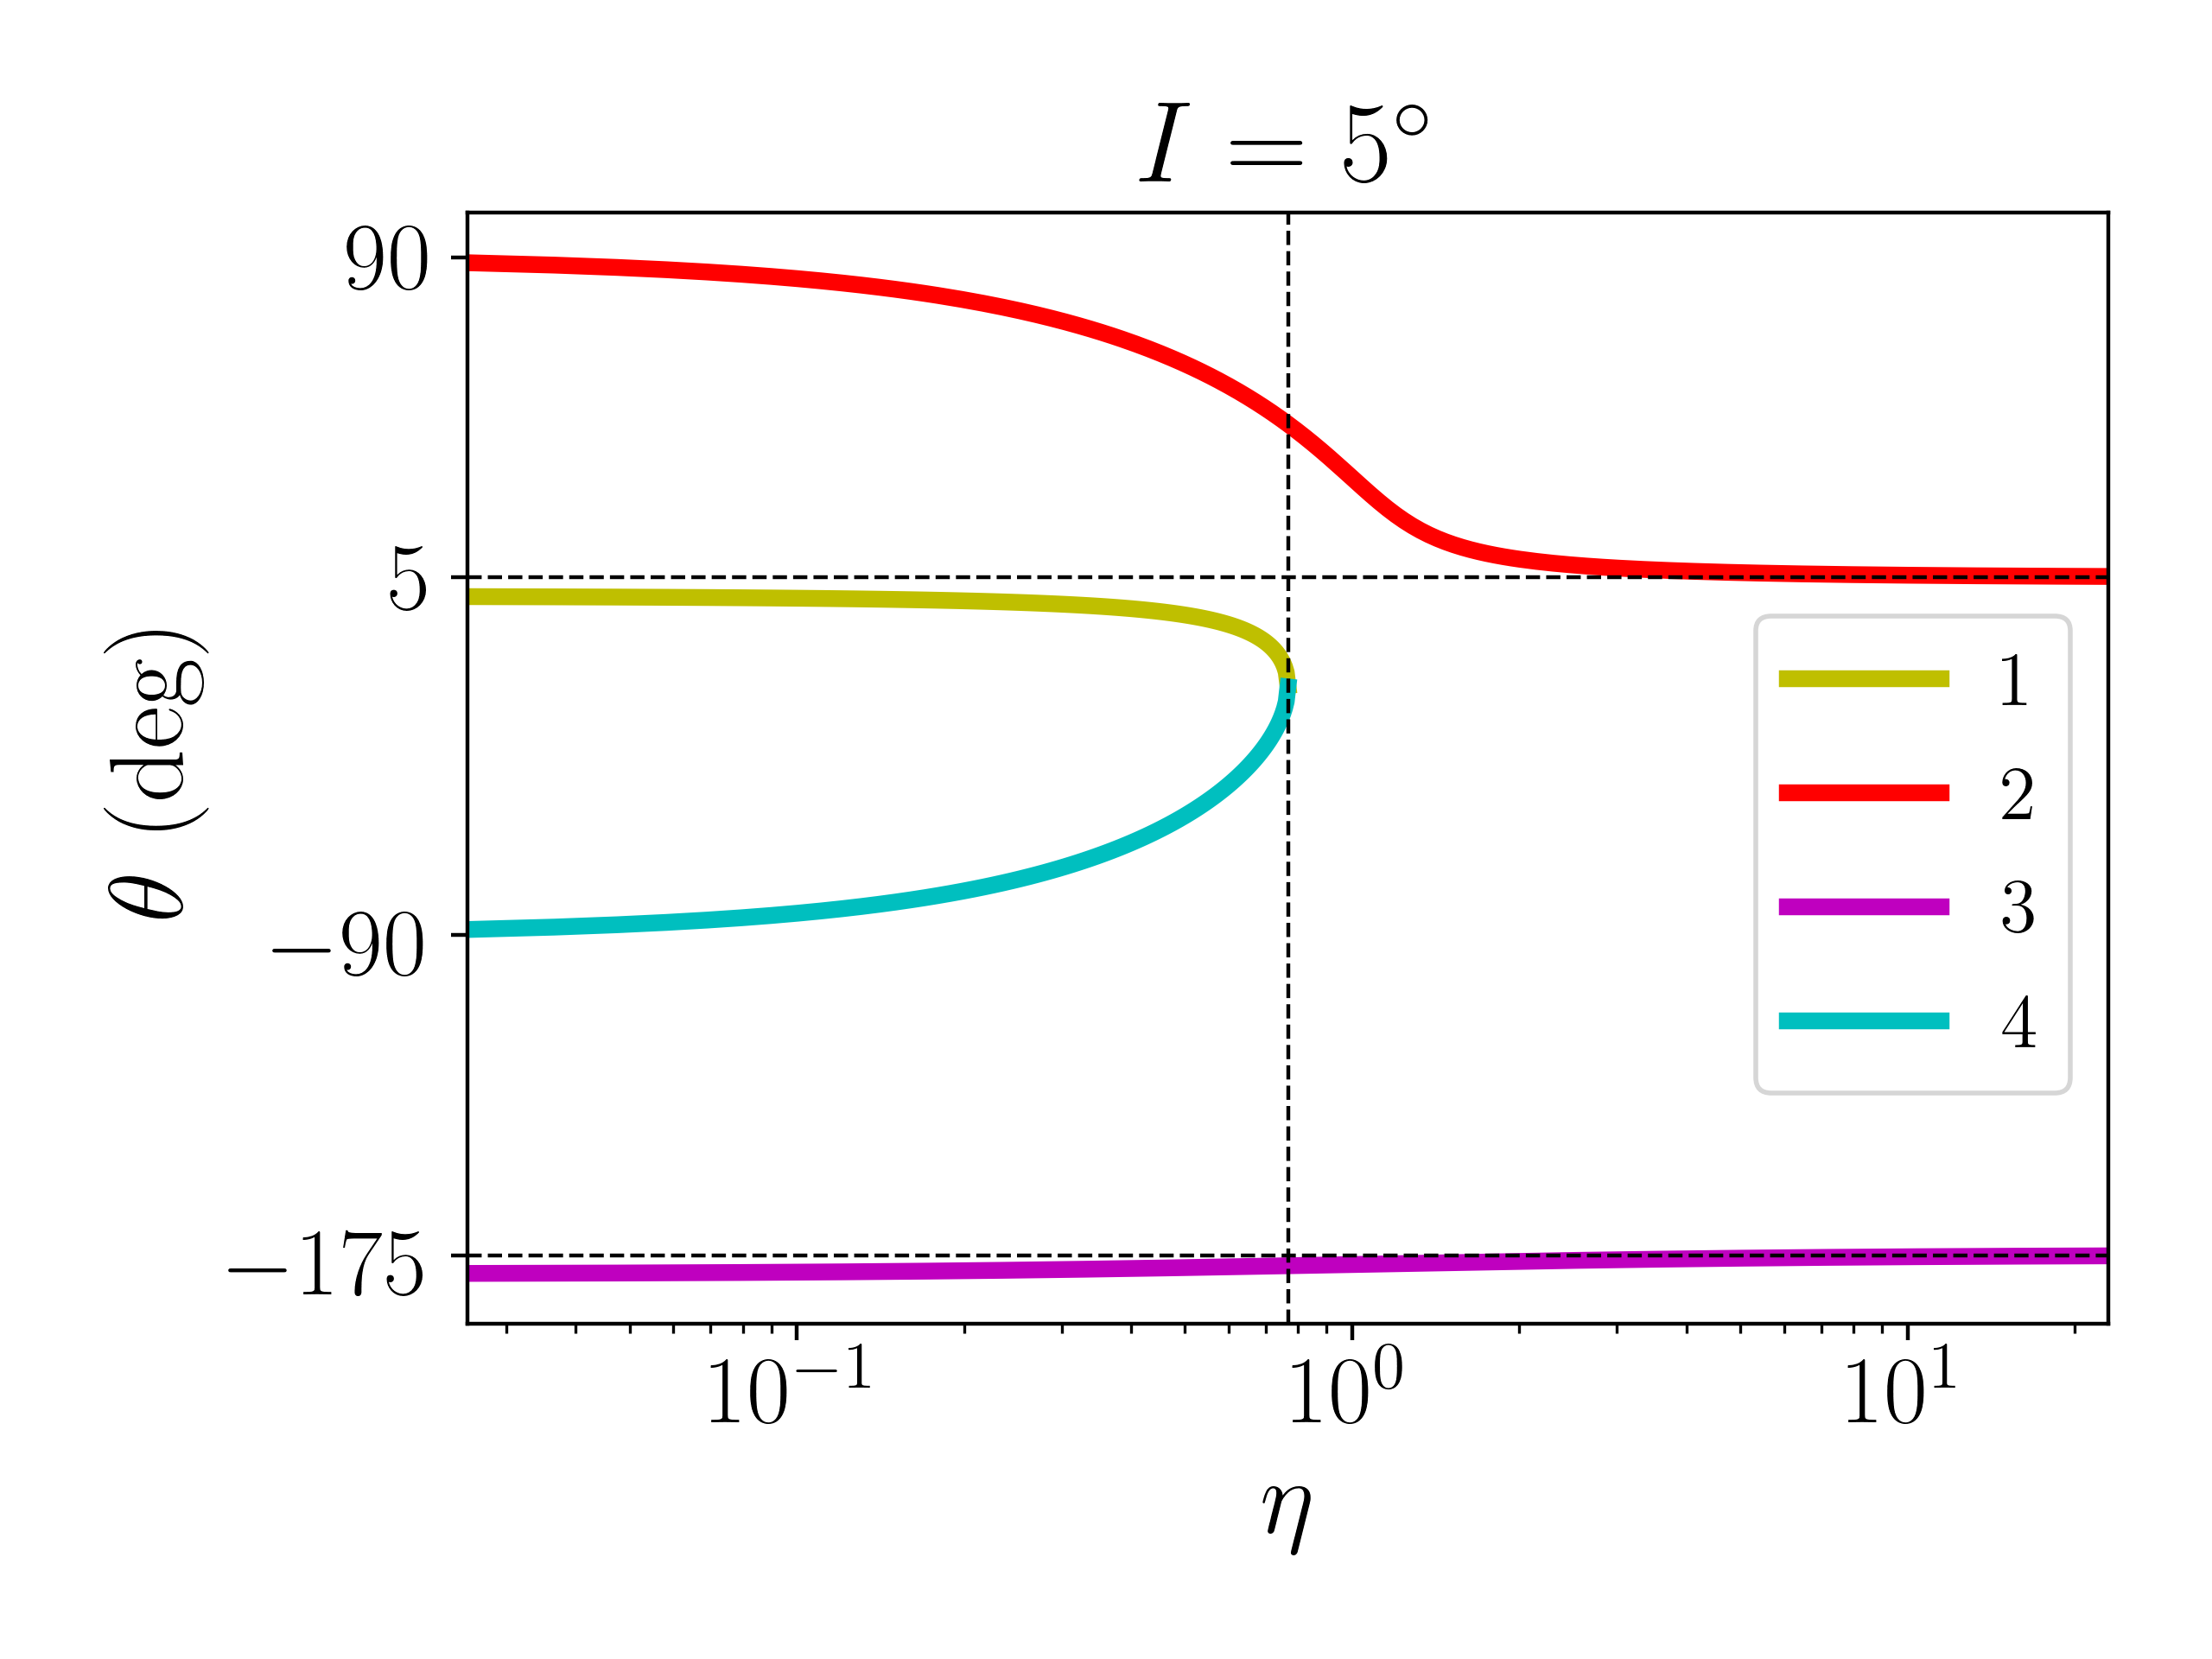
\includegraphics[width=\columnwidth]{../initial/99_misc/2_cs_locs.png}
    \caption{CS locations, TODO change axis labels etc.}\label{fig:cs_locs}
\end{figure}

Note that $\phi$ is conjugate to $\cos \theta$, and thus the spin dynamics
obey Hamiltonian:
\begin{equation}
    H(\mu, \phi; s) = -\frac{s}{s_{\rm c}}\frac{\mu^2}{2}
        + \mu \cos I - \sin I \sqrt{1 - \mu^2}\cos \phi.
\end{equation}

Plot of level curves of Hamiltonian as before, including $\mathcal{C}_{\pm}$
notation in Fig.~\ref{fig:1contours}.
\begin{figure}
    \centering
    \includegraphics[width=\columnwidth]{../initial/0_eta/1contours.png}
    \caption{TODO label $\mathcal{C}_{\pm}$.}\label{fig:1contours}
\end{figure}

\subsection{Weak Tidal Friction}\label{ss:weak_tides}

We implement the weak friction theory of equilibrium tides \citep{lai2012},
under which both $\theta$ and $s$ evolve. We define the dimensionless time
\begin{equation}
    \tau \equiv gt.
\end{equation}
The full equations of motion including weak tidal friction are then
\begin{align}
    \rd{\uv{s}}{\tau}
        ={}& \frac{s}{s_c}\p{\uv{s} \cdot \uv{l}}\p{\uv{s} \times
                \uv{l}} - \uv{s} \times \uv{l}_{\rm p}\nonumber\\
            &+ \frac{\epsilon 2n}{s}
                \p{1 - \frac{s}{2n}\p{\uv{l} \cdot \uv{s}}}
                    \uv{s} \times \p{\uv{l} \times \uv{s}},\\
    \rd{s}{\tau}
        ={}& \epsilon 2n \p{\uv{s} \cdot \uv{l} -
            \frac{s}{2n}\p{1 + \p{\uv{s} \cdot \uv{l}}^2}},
\end{align}
where $\epsilon$ measures the tidal dissipation rate and is given by
\begin{align}
    \epsilon &\equiv -\frac{1}{gt_a}\frac{L}{2S} \frac{s}{2n},\\
    \frac{1}{t_a} &= \frac{3k_2}{Q}\p{\frac{m}{M}}\p{\frac{R}{a}}^5 n.
\end{align}
Here, $L$ and $S$ are the orbital and spin angular momenta of the inner planet,
respectively.

The phase portrait for these EOM in $\p{s, \theta}$ space is shown in
Fig.~\ref{fig:quiver}.
\begin{figure}
    \centering
    \includegraphics[width=\columnwidth]{../initial/1_weaktide/2quiver0_2.png}
    \caption{Phase portrait.}\label{fig:quiver}
\end{figure}
Note that the semimajor axis $a$ is not constant, but $\dot{a} / \dot{\theta}
\sim S / L \ll 1$, and is negligible for our problem (but not always,
Millholland tidal runaway cite).

\subsection{Stable Equilibria of Tidal Friction}\label{ss:tidal_eqs}

Generally, these EOM have equilibria at the points that are both a CS and
satisfy $\dot{s} = 0$ under weak tidal friction. These are stable when ignoring
tidal friction \citep{su2020}. On Fig.~\ref{fig:quiver}, these are the
intersection of the locations of CS1 and CS2 with the line $\dot{s} = 0$. It is
clear that the locations of these equilibria depend on the value of $s_c$. Call
these generalized equilibria \emph{tidal Cassini Equilibria} (tCE), and number
them tCE1 and tCE2 depending on whether they are CS1 or CS2 states. Shown
\begin{figure}
    \centering
    \includegraphics[width=\columnwidth]{../initial/1_weaktide/6equils0_06.png}
    \caption{Location of tCE\@. Vertical line is spin rate below which tCE is
    destroyed.}\label{fig:6equils}
\end{figure}

Furthermore, if tides are too strong (large $\epsilon$), tCE2 can become
unstable (cite Fabrycky). The required $\epsilon$ for stability of tCE2 is given
by
\begin{equation}
    \epsilon \leq \frac{\eta_2 \sin I}{1 - \mu_2^2},
\end{equation}
where $\eta_2$ and $\mu_2$ are evaluated at tCE2.

\section{Probability Distribution of Outcomes}\label{s:sim}

The general question of the dynamics is then as follows: given problem
parameters (including $s_c$) and an initial planet spin and obliquity $(s,
\theta)$, what are the possible outcomes and their associated probabilities? We
study this first at fixed $s_c$ as a function of $\theta$ in
Section~\ref{ss:q_dist}, then as a function of $s_c$ for an isotropic initial
spin $\hat{s}$ in Section~\ref{ss:s_c_dist}.

\subsection{Distribution As a Function of $\theta$}\label{ss:q_dist}

As a result of Section~\ref{ss:tidal_eqs}, the tCE are the only possible final
outcomes. We generate initial spin vectors $\hat{s}$ for isotropic initial
distribution $\p{\cos \theta, \phi}$, and average over $\phi$ in histograms.
This gives histograms in
Figs.~\ref{fig:Hhists_0_06,fig:Hhists_0_20,fig:Hhists_0_70}
\begin{figure}
    \centering
    \includegraphics[width=\columnwidth]{../initial/1_weaktide/5Hhists0_06_5.png}
    \caption{$s_c = 0.06$. Note that it is difficult to reach
    tCE2.}\label{fig:Hhists_0_06}
\end{figure}
\begin{figure}
    \centering
    \includegraphics[width=\columnwidth]{../initial/1_weaktide/5Hhists0_20_5.png}
    \caption{$s_c = 0.2$. Note that tCE2 is both reached with substantial
    probability and has substantial obliquity.}\label{fig:Hhists_0_20}
\end{figure}
\begin{figure}
    \centering
    \includegraphics[width=\columnwidth]{../initial/1_weaktide/5Hhists0_60_5.png}
    \caption{$s_c = 0.6$. Note that tCE2 becomes attracting over tCE1, but will
    have obliquity $\approx I$ and is uninteresting.}\label{fig:Hhists_0_70}
\end{figure}

Similarly to \citet{su2020}, these probabilities are the result of separatrix
crossings. However, the calculation differs from \citet{su2020}: since the
perturbation is dissipative in phase space (i.e.\ it does not conserve phase
space area), analysis following \citet{henrard1982} is not sufficient. A more
general theory of separatrix crossing is still able to predict the outcome
probabilities. Appendix~\ref{app:probs} gives a more thorough overview of
separatrix crossing dynamics, but the key result is:
\begin{equation}
    a^2 + b^2 = c^2.
\end{equation}
We can apply this curve to calculate the likelihood of the tCEs when a
particular trajectory encounters the separatrix, and from this obtain a
semi-analytical prediction of the distribution of outcomes. The semi-analytical
nature of this calculation arises because $\eta_\star$ cannot be calculated
\emph{a priori}. The agreement of this curve with the histograms is examined for
the same three $s_c$ values in
Figs.~\ref{fig:pc_fits_0_06,fig:pc_fits_0_20,fig:pc_fits_0_70}.
\begin{figure}
    \centering
    \includegraphics[width=\columnwidth]{../initial/1_weaktide/5pc_fits0_06_5.png}
    \caption{$s_c = 0.06$ prediction vs histogram.}\label{fig:pc_fits_0_06}
\end{figure}
\begin{figure}
    \centering
    \includegraphics[width=\columnwidth]{../initial/1_weaktide/5pc_fits0_20_5.png}
    \caption{$s_c = 0.20$ prediction vs histogram.}\label{fig:pc_fits_0_20}
\end{figure}
\begin{figure}
    \centering
    \includegraphics[width=\columnwidth]{../initial/1_weaktide/5pc_fits0_70_5.png}
    \caption{$s_c = 0.70$ prediction vs histogram.}\label{fig:pc_fits_0_70}
\end{figure}

\subsection{Distribution As a Function of $s_c$}\label{ss:s_c_dist}

Assuming that $\hat{s}$ is drawn from an isotropic distribution, we may then
calculate the probabilities of going to either tCE as a function of $s_c$. This
is shown below for $I = 5^\circ$
\begin{figure}
    \centering
    \includegraphics[width=\columnwidth]{../initial/1_weaktide/5probs_5.png}
    \caption{Top: total probability of ending up in tCE2 (blue dots) and the
    prediction ignoring separatrix capture (red line). Bottom:
    obliquities of the tCEs.}\label{fig:probs}
\end{figure}

Note that while only the results for an isotropic distribution of initial
$\hat{s}$ are shown, in principle arbitrary distributions $P\p{\theta_i}$ can be
convolved against the $P_{tCE2}\p{\theta_i}$ distributions shown in
Section~\ref{ss:q_dist}.

\section{Summary and Discussion}\label{s:summary}

\bibliography{Su_weak_tides}
\bibliographystyle{aasjournal}

\appendix

\section{Separatrix Crossing Dynamics}

\subsection{Theory}\label{app:sep_crossing_dynamics}

\subsubsection{Application of Adiabatic Invariance: Henrard Theory}

Review Henrard result, is already very successful e.g.\ MMR capture.

\subsubsection{Melnikov Integral}\label{sss:Melnikov}

The first substantial new result.

\subsubsection{Example: Constant $s$}

``Toy problem 1'', the nice $P_c \propto \eta^{3/2}$ result. Application of
Section~\ref{sss:Melnikov}.

\subsubsection{Combined Result}

Thus, the natural extension of the two above results should be
\begin{align}
    \Delta_{\pm} &= \oint_{\mathcal{C}_{\pm}} \rd{H}{t}\;\mathrm{d}t,\\
        &= \oint_{\mathcal{C}_{\pm}}
            \dot{\mu}^{(1)} + \frac{\dot{s}^{(1)}}{\dot{\phi}^{(0)}}
                \p{\pd{H}{s} - \pd{H_4}{s}}\;\mathrm{d}\phi.
\end{align}

\subsection{Separatrix Crossing Probability: Tidal Friction}\label{app:probs}

Application of the full formula presented in
Section~\ref{app:sep_crossing_dynamics}. The key result is that one integrates
\begin{equation}
    \rd{(\Delta H)}{(\epsilon t)} \approx
            (1 - \mu^2)\p{\frac{2\Omega}{s} - \mu}
                \dot{\phi}^{(0)} + 2\Omega\p{1 + \frac{s}{2\Omega}(1 + \mu^2)}
                \s{\frac{\mu^2}{2s_c} - \frac{s_c}{2s^2}\cos^2 I}.
\end{equation}

An analytical form that holds when $s \gg s_c$ is:
\begin{align}
    \frac{\Delta_{\pm}}{\epsilon} ={}&
        -2\cos I\p{\pm 2\pi \eta \cos I + 8\sqrt{\eta \sin I}}
        \pm 2\pi s\cos I
        + \eta \cos I \p{-8\sqrt{\sin I / \eta}}
            + \frac{s}{2}8\sqrt{\sin I/\eta}\nonumber\\
        &+ \frac{2\Omega}{s}\p{\mp 2\pi\p{1 - 2\eta \sin I}
            + 16\cos I \eta^{3/2}\sqrt{\sin I}}
            + 8\sqrt{\eta \sin I}
            \pm 2 \pi \eta \cos I
            - \frac{64}{3} \p{\eta \sin I}^{3/2}.
\end{align}
The capture probability is then just
\begin{equation}
    P_c = \frac{\Delta_+ + \Delta_-}{\Delta_-}.
\end{equation}

\end{document}
